\chapter{Úvod}
Současný život je ze všeho nejvíce závislý na informacích - na jejich získávání, zpracování, předávání - jednoduše informace ovlivňují veškerý náš život 
a nedovedeme si naší existenci představit jinak. 
Jelikož je dnešní svět neodmyslitelně spjat s počítači a internetem, je zřejmé, že velkou část informací dnes vnímáme právě skrze počítač a zejména díky internetu.
Díky těmto skutečnostem potřebujeme mít k dispozici fungující principy vyhledávání v neustále se zvětšujícím počtu informací.

World Wide Web (WWW) - dále jen Web - byl zpočátku navržen a využíván ve své podstatě jako obrovská databáze dokumentů (tj. webových prezentací, souborů, aplikací aj.), které na sebe vzájemně odkazují \cite{www}. 
Mezi jednotlivými dokumenty přecházíme díky jejich propojení s dalšími dokumenty pomocí hypertextu\footnote{Hypertext je text zobrazený uživateli, který obsahuje odkazy (reference) na další obsah, který je ihned přístupný obvykle kliknutím myši. Pojem vymyslel Ted Nelson v roce 1965. Zdroj \cite{hypertext}}. 
Síla odkazů tedy je v komplexním propojení doslova čehokoliv s čímkoliv. Zároveň je to ale nevýhoda - velmi snadno lze při velkém množství odkazů ztratit přehled. Čím více existuje na webu dokumentů, tím je více odkazů a tím je také složitější dostat se rychle a přímo k hledané informaci.
Web byl od svého vzniku vytvářen převážně pro uživatele, z toho důvodu bohužel počítač, resp. prohlížeč webových dokumentů (dále jen prohlížeč), nerozumí dokumentům stejným způsobem jako lidé, neví, co který obsah znamená a tudíž nezná ani souvislosti mezi dokumenty (obr. \ref{img:hyperlinks}). 
Všechna propojení jsou vytvořena pouze přímo autory dokumentů.

\begin{figure}[h]
\begin{center}
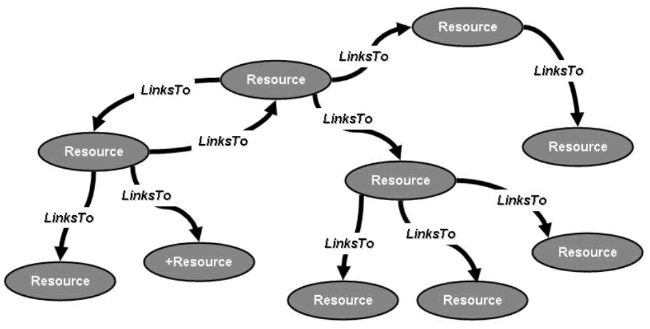
\includegraphics[width=12cm]{figures/hyperlinks}
\caption{Schéma tradiční struktury webu tak, jak ji chápe počítač. (Zdroj \cite{holyj_webexpo})}
\label{img:hyperlinks}
\end{center}
\end{figure}

Web 2.0 (název pro aktuální stav či úroveň webových technologií) se snaží uživatele více zapojit do vytváření samotného obsahu. Předtím mohl uživatel web de facto pouze číst, nyní je mu poskytnuta určitá míra interaktivity pomocí blogů, wikipedií, sociálních sítí, mash-upů\footnote{Mash-up je webová aplikace, která vytváří nové služby pomocí kombinování funkcionalit z více zdrojů \cite{mashup}, např. použitím různých Application programming interface (API).}, tagování, Rich Internet Application (RIA)\footnote{RIA jsou webové aplikace podobající se charakterem aplikacím desktopovým. Za pomoci různých RIA nástrojů umožňují vysokou míru interakce a uživatelského prožitku \cite{ria}.} atp.
Stále se však používá stejný princip vyhledávání, tj. pomocí fulltextového vyhledávání, skrze klíčová slova, kdy se prochází každý dokument a ve výsledku se zobrazí relevantní odkazy na příslušné dokumenty, které obsahují hledané slova. Jinými slovy počítač stále nerozumí obsahu.

\section{Sémantika}

Vznikla tedy potřeba zachytit sémantiku informací uvedených ve webových dokumentech, aby s těmito informacemi mohl počítač dále pracovat na vyšší úrovni, než jen na úrovni fulltextového vyhledávání. 
Sémantiku definuje lingvistika jako nauku o významu slov a znaků \cite{semantics}, v souvislosti s webem tedy chápeme sémantiku jako význam informace.
Tento postup vede ke změně chápání přístupu k webového obsahu a na zcela jinou úroveň posunuje schopnosti a možnosti webových vyhledávačů. Za ideální stav (tedy za stav, jehož se pokoušíme dosáhnout) je považován okamžik, kdy počítač zcela dokáže pochopit náš přirozený jazyk. \cite{europen}.

Od připojování dodatečných informací (tzv. metadata), popisujících původní data, přes přiřazování vazeb a vlastností mezi jednotlivými daty až po zpracovávání znalostních databází určitého objektu tedy směřuje budoucí vývoj webu k porozumění počítače lidskému chápání \cite{web30}.

Pro webové dokumenty nejčastěji vytvářené pomocí (eXtensible) HyperText Markup Language (HTML, XHTML), což je jazyk pro vytváření šablon webových dokumentů, se ustálil pojem Plain Old Semantic HTML (POSH), který vznikl z praktickým důvodů; moderní vývoj webu neustále zmiňuje a zdůrazňuje pojmy jako validita, beztabulková úprava, správná sémantika a vše související. Pokaždé opakovat všechny tyto pěvně svázané pojmy je zdlouhavé (naopak ale potřebné), proto vznikl pojem POSH, který všechny tyto pojmy nahrazuje a zaštiťuje. \cite{posh}
Sémantika jazyka HTML pouze říká, že v dokumentu jsou např. odstavce, nadpisy, seznamy apod., již ale neudává, že např. první buňka tabulky značí název produktu a druhá jeho cenu \cite{europen}.

Extensible Markup Language (XML) odstraňuje tento sémantický nedostatek díky využívání vlastních specifických značek, které udávají význam informace (sémantické značkování). Bohužel se XML (ve své čisté podobě) pro zachycování sémantiky na webu v širší praxi příliš neujalo \cite{europen}. 

Pro zlepšení sémantiky ve webovém prostředí se hojně začali využívat tzv. mikroformáty, které s sebou přinesl Web 2.0. Využívají existující jazyk (X)HTML novým způsobem resp. do kódu vhodně doplňují strukturované informace (vizitky, události aj.) \cite{microformat}.
Jednoduchost začlenění mikroformátů do webové stránky zapříčinila v praxi jejich hojné využívání.
Nicméně stále se jedná jen o jednoduché rozšíření sémantiky HTML, resp. nyní je počítač schopen rozeznat např. co je telefonní číslo a co jméno osoby, tím to ale také končí; není možné z těchto dat cokoliv odvozovat, nelze mezi daty hledat souvislosti.

\section{Sémantický web}

Na scénu proto nastupují technologie, které mají za cíl, aby počítače dokázali chápat význam jednotlivých dat a dokázali mezi nimi hledat spojitosti podobným způsobem, který je lidem přirozený. Takové technologie se souhrnně označují jako \textit{Sémantický web}.
Výsledek Sémantického webu si pro začátek můžeme předtavit jako graf věcí a vztahů, viz obr. \ref{img:futureWebSchema} 

\begin{figure}[h]
\begin{center}
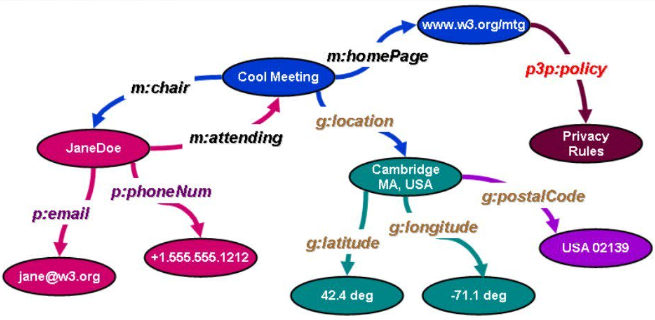
\includegraphics[width=12cm]{figures/futureWebSchema}
\caption{Schéma sémantické struktury webu, který ukazuje jeden ze základních cílů Sémantického webu. (Zdroj \cite{holyj_webexpo})}
\label{img:futureWebSchema}
\end{center}
\end{figure}

Účelem Sémantického webu, nazývaného také jako Web of Data či Web 3.0, je popis věcí a vytváření vztahů mezi nimi, formulace internetových dat tak, aby byly srozumitelné i pro počítače, tj. nejen pro lidi \cite{zdrojakSemWeb}.   
Sémantický web vytváří společný formát pro interakci a kombinaci dat mezi různými zdroji. Dále Sémantický web zachycuje, jakým způsobem data souvisí s objekty reálného světa \cite{semWeb}.

Součástí Sémantického webu je tzv. \textit{znalostní báze}. Znalostní báze reprezentuje určitou znalostní doménu \cite{kunc}. Např. pro doménu hudby tedy znalostní báze obsahuje objekty z reálného světa relevantní k hudbě, což je např. interpret, kabela, album, žánr atp., a dále vztahy mezi nimi. Shromáždíme-li všechny tyto věci související s hudbou na jedno místo, získáme tak doménu znalostí vyjádřenou znalostní bází.
Pro popis struktury znalostní báze se používají ontologie \cite{obitko}, často definované jako explicitní specifikace konceptualizace\footnote{Konceptualizace je systém pojmů modelující určitou část světa.} \cite{gruber}.
Architekturu Sémantického webu popisuje obrázek \ref{diagram:SemWebArch}, který ukazuje jak jsou technologie standardizované pro Sémantický web organizovány a dále ukazuje, že Sémantický web rozšiřuje, nikoli nahrazuje, klasický hypertextový web. Diagram je stále ve vývoji, jelikož zdaleka ne všechny vrstvy jsou dnes standardizovány - vrchní vrstvy jsou zatím návrhy, které je potřeba teprve implementovat \cite{semWebStack}.

\section{Vymezení cílů a požadavků}  

Jedním z oborů, kde se v současné době začínají ontologie používat, je hudební průmysl. 
Cílem této práce je navrhnout a vytvořit základní ontologii, která popíše doménu hudby.
Požadavkem pro úspěšné vytvoření ontologie je znalost nástrojů na tvorbu ontologií, proto je nutné před samotným návrhem možnosti těchto nástrojů zanalyzovat.

Tato ontologie propojí a vytvoří reálné souvislosti mezi jednotlivými interprety, žánry, apod. 
Počítač tak bude schopen s těmito informacemi zacházet podobným způsobem, jakým s nimi pracuje člověk.  
K tomu je však potřeba nad touto ontologií vytvořit vyhledávací systém, do kterého bude uživatel vkládat své dotazy.
Vyhledávací systém vytvořený v této práci bude uživateli nabízet odpovědi na otázky typu "líbí se mi zpěvák Bobby McFerrin, ukaž mi jemu podobnou hudbu". Systém tedy bude nabízet podobnou hudbu. 

Výsledek práce bude sloužit jako jádro nabízecího systému pro hudební přehrávač \cite{kunc}.

\section{Struktura práce}

Tato práce je rozdělena do 6ti kapitol. 1. kapitola čtenáře uvadí do kontextu a motivuje k vytváření Sémantického webu.
2. kapitola vysvětluje, co jsou ontologie, k čemu slouží a jak se vytvářejí.
Kapitola 3. analyzuje vytvoření ontologie hudby a strukturu webové aplikace.
4. kapitola seznamuje s implementačním prostředím, 5. kapitola poskytuje výsledky testování systému. 
Konečně kapitola 6. práci uzavírá a diskutuje budoucí rozšíření.